\qns{Page Rank}

\textbf{Learning Goal:} This problem is designed to provide insight into state transition. We will observe how the steady state depends of the eigenvalue and eigenvectors of a state-transition matrix.
% author: Aditya Baradwaj
% email: abaradwaj@berkeley.edu

% \begin{enumerate}[label=(\alph*)]
%     \item Prove that any matrix and its transpose have the same eigenvalues. I.e. suppose you have some matrix $\m{A}$. Prove that A and $\m{A}^T$ have the same eigenvalues. \textit{Hint: Recall that the eigenvalues of a matrix can be found by solving the equation $det(\m{A} - \lambda \m{I}) = 0$, and that a matrix and its transpose have the same determinant}
    
%     \meta{
%     Students will probably be new to the 'volume of a parallelipiped' interpretation of the determinant. So it might be a good idea to go through this with them, instead of asking them to try and solve it.
%     }
    
%     \ans{
%     The eigenvalues of $\m{A}$ are the solutions to the equation $det(A - \lambda I) = 0$. A matrix and its transpose will have the same determinant, because they represent the same transformation, except they rotate in opposite directions but keep the same scaling, and therefore the same volume is enclosed by the parallelepiped. This means that
%     $$det((\m{A} - \lambda \m{I})^T) = 0 \implies det(\m{A}^T - \lambda \m{I}^T) = 0 \implies det(\m{A}^T - \lambda \m{I}) = 0$$. But this equation gives us the eigenvalues of $\m{A}^T$! And since we have proved that these equations are the same, so their solutions must be the same, and the eigenvalues must also be the same.
%     }
% \end{enumerate}

Now suppose we have a network consisting of 3 websites connected as shown below. Each of the weights on the edges represent the probability of a user taking that edge.

\usetikzlibrary{positioning}
\definecolor {processblue}{cmyk}{0.96,0,0,0}

\begin{center}
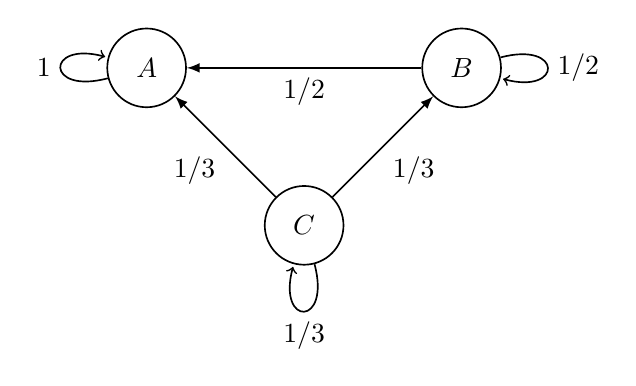
\begin{tikzpicture}[-latex, auto, node distance= 2cm and 2cm , on grid, semithick, state/.style ={circle, draw, minimum width=1 cm}]

\node[state] (C) {$C$};
\node[state] (A) [above left=of C] {$A$};
\node[state] (B) [above right =of C] {$B$};
\path (A) edge [loop left] node[left] {$1$} (A);
\path (C) edge node[below left] {$1/3$} (A);
\path (C) edge node[below right] {$1/3$} (B);
\path (C) edge [loop below] node[below] {$1/3$} (C);
\path (B) edge [loop right] node[right] {$1/2$} (B);
\path (B) edge node[below] {$1/2$} (A);
\end{tikzpicture}
\end{center}

\begin{enumerate}
    \item Call the transition matrix for this system $\mathbf{P}$ Write down $\mathbf{P}$ from this graph.  (\textit{Hint: Try to recall the properties of transition matrices and observe the sum of each column}).
    
\meta{
    \begin{itemize}
   	\item Explain that the columns of the transition matrix summing to 1 indicate that the system is conservative, i.e. no elements are being added to or removed from the system.
   	\item  You can discuss the mechanical solutions to each of these problems, but also emphasize that applying a conceptual understanding of state transition matrices allows you to solve each part of this problem with very little actual linear algebra.
    \end{itemize}
}

 
    
    \ans{
    
    Transition matrix notation: Let $A\rightarrow B$ represent the fraction of $A$ that goes to $B$ after transition. Then, a general $3\times3$ transition matrix with states $A$, $B$, and $C$ can be written as follows: \\

    $$\begin{bmatrix}
    A \rightarrow A & B \rightarrow A & C \rightarrow A \\  
    A\rightarrow B & B\rightarrow B & C\rightarrow B \\
    A \rightarrow C & B \rightarrow C & C \rightarrow C \\
    \end{bmatrix}$$


    The transition matrix is:
    $$\mathbf{P}=\begin{bmatrix}
    1 & \frac{1}{2} & \frac{1}{3} \\
    0 & \frac{1}{2} & \frac{1}{3} \\
    0 & 0 & \frac{1}{3} \\
    \end{bmatrix}$$
    
    }
    
    \item We want to rank these webpages in order of importance. Can you predict at least one of the eigenvalues of $\mathbf{P}$? Verify your predicted eigenvalue by calculation and then find the corresponding eigenvectors of $\mathbf{P}$.
    

    


    \ans{
    
    We see that the columns of the transition matrix sum to $1$. This means that population is conserved in this system, and the system might reach a steady-state. This hints that $\lambda_1=1$ might be an eigenvalue of the matrix $\mathbf{P}$.
    
    \begin{align*}
    \mathbf{P}\vec{v_1}&=\lambda_1\vec{v_1}\\
    \mathbf{P}\vec{v_1}&=\lambda_1\mathbf{I}\vec{v_1}\\
        (\mathbf{P}-\lambda_1\mathbf{I})\vec{v_1}&=\vec{0}\\
        (\mathbf{P}-\mathbf{I})\vec{v_1}&=\vec{0}\\
   (\begin{bmatrix}
    1 & \frac{1}{2} & \frac{1}{3} \\
    0 & \frac{1}{2} & \frac{1}{3} \\
    0 & 0 & \frac{1}{3} \\
    \end{bmatrix}
    - \begin{bmatrix}
    1 & 0 & 0 \\
    0 & 1 & 0 \\
    0 & 0 & 1 \\
    \end{bmatrix})\vec{v_1} &= \vec{0}\\
       \begin{bmatrix}
    0 & \frac{1}{2} & \frac{1}{3} \\
    0 & -\frac{1}{2} & \frac{1}{3} \\
    0 & 0 & -\frac{2}{3} \\
    \end{bmatrix}
    \vec{v_1} &= \vec{0} \\
       \begin{bmatrix}
    0 & \frac{1}{2} & \frac{1}{3} \\
    0 & 0 & \frac{2}{3} \\
    0 & 0 & -\frac{2}{3} \\
    \end{bmatrix}
    \vec{v_1} &= \vec{0} \mbox{\quad using $R_2 \leftarrow R_2 + R_1$}\\
       \begin{bmatrix}
    0 & \frac{1}{2} & \frac{1}{3} \\
    0 & 0 & \frac{2}{3} \\
    0 & 0 & 0 \\
    \end{bmatrix}
    \vec{v_1} &= \vec{0} \mbox{\quad using $R_3 \leftarrow R_3 + R_2$}\\
    \end{align*}
    We can see that the pivots lie in the second and third columns. So, we want to solve the equation:
    \begin{flalign*}
    & \begin{bmatrix}
    0 & -\frac{1}{2} & \frac{1}{3} \\
    0 & 0 & -\frac{2}{3} \\
    0 & 0 & 0 \\
    \end{bmatrix}
    \begin{bmatrix} x_1 \\ x_2 \\ x_3 \end{bmatrix} = \vec{0} &\\
    & \implies -\frac{1}{2}x_2 + \frac{1}{3}x_3 = 0 \text{ and } -\frac{2}{3}x_3 = 0 &\\
    & \implies x_3 = 0 \text{ and } x_2 = 0
    \end{flalign*}
    This means that the eigenvector is of the form $\begin{bmatrix}x_1 \\ 0 \\ 0\end{bmatrix} = \begin{bmatrix}1 \\ 0 \\ 0\end{bmatrix}x_1$. And since $x_1$ is a free variable, the eigenvectors corresponding to eigenvalue $1$ must belong in $\textrm{span}\left\{ \begin{bmatrix}1 \\ 0 \\ 0 \end{bmatrix}\right\} $.
    }
    
    
    \item Now you are told that the other two eigenvalues of $\mathbf{P}$ are $\lambda_2=\frac{1}{2}$ and $\lambda_3=\frac{1}{3}$, and the corresponding eigenvectors are $\vec{v_2}=\begin{bmatrix}1 \\ -1 \\ 0 \end{bmatrix}$ and $\vec{v_3}=\begin{bmatrix}1 \\ -2 \\ 1 \end{bmatrix}$, respectively.\\
Suppose we start with just $30$ users in $A$ and no users in $B$ and $C$. Can you express the initial state, $\vec{x}[0]$, as a linear combination of $\vec{v_1}$, $\vec{v_2}$ and $\vec{v_3}$?    

    \meta{
    \begin{itemize}
  
    \item Students also have NOT learned how to calculate the determinant of a 3 by 3 matrix. Finding the eigenvalues of a 3 by 3 matrix is \textbf{out of scope} unless it is a diagonal matrix. 
    \end{itemize}
    
}
    
    \ans{
    
    The initial vector of users is $\vec{x}[0] = \begin{bmatrix}30 \\ 0 \\ 0\end{bmatrix}$. We assume
    \begin{align*}
    \vec{x}[0]=\alpha_1\vec{v_1}+\alpha_2\vec{v_2}+\alpha_3\vec{v_3},
    \end{align*}
    where $\alpha_1$, $\alpha_2$ and $\alpha_3$ are scalars.
    We can see by inspection that $\alpha_1=30$, $\alpha_2=0$ and $\alpha_3=0$ for this problem.
    }
    
    \item Now use the results from the previous part to express the state at time step $n$ as a function of the eigenvectors and eigenvalues. What is the steady-state? Is the steady-state different from the initial state? Why? \\ 
    \textbf{Relevant Notes:} \notes{ Note 9: Subsection 9.8.2} are helpful for this problem.
    \ans{
  \begin{align*}
    \vec{x}[0]&=\alpha_1\vec{v_1}+\alpha_2\vec{v_2}+\alpha_3\vec{v_3}\\
    \vec{x}[1]&=\mathbf{P}\vec{x}[0]=\alpha_1\mathbf{P}\vec{v_1}+\alpha_2\mathbf{P}\vec{v_2}+\alpha_3\mathbf{P}\vec{v_3}=\alpha_1\lambda_1\vec{v_1}+\alpha_2\lambda_2\vec{v_2}+\alpha_3\lambda_3\vec{v_3}\\
    \vec{x}[2]&=\mathbf{P}\vec{x}[1]=\alpha_1\lambda_1\mathbf{P}\vec{v_1}+\alpha_2\lambda_2\mathbf{P}\vec{v_2}+\alpha_3\lambda_3\mathbf{P}\vec{v_3}=\alpha_1\lambda_1^2\vec{v_1}+\alpha_2\lambda_2^2\vec{v_2}+\alpha_3\lambda_3^3\vec{v_3}\\
    \hdots\\    
        \vec{x}[n]&=\alpha_1\lambda_1^n\vec{v_1}+\alpha_2\lambda_2^n\vec{v_2}+\alpha_3\lambda_3^n\vec{v_3}\\
        \vec{x}[n]&=30\lambda_1^n\vec{v_1}+0\lambda_2^n\vec{v_2}+0\lambda_3^n\vec{v_3}=30(1)^n\begin{bmatrix}
    1\\ 0 \\ 0
    \end{bmatrix}=\begin{bmatrix}
    30\\ 0 \\ 0
    \end{bmatrix}
    \end{align*}  
    
    The steady state is given by:
    \begin{align*}
    \vec{x}_{steady}=\lim_{n \to +\infty}30(1)^n\begin{bmatrix}
    1\\ 0 \\ 0
    \end{bmatrix}=\begin{bmatrix}
    30\\ 0 \\ 0
    \end{bmatrix}
    \end{align*} 
 The steady state is the same as the initial state, because the initial state vector is in the eigenspace corresponding to $\lambda_1=1$, i.e. it is in the direction of $\vec{v_1}$.   
    }
    
        \item Now suppose we start with $30$ users in $A$, $30$ users in $B$ and no users in $C$. Express the initial state, $\vec{x}[0]$, as a linear combination of $\vec{v_1}$, $\vec{v_2}$ and $\vec{v_3}$ and find the steady state. Is the steady-state different from the initial state? Why?
        
\meta{
\begin{itemize}

\item Explain that the initial state has three components in the direction of three eigenvectors. 

\item Mention how each component reacts to the transition. 

\item Remind the students that expressing the initial state $\vec{x}[0]$ as a linear combination of $\vec{v_1}$, $\vec{v_2}$,  and $\vec{v_3}$ means finding coefficients $\alpha_1$,  $\alpha_2$, and $\alpha_3$  so that $\vec{x}[0]$ is in the span of the eigenbasis formed by $\vec{v_1}$, $\vec{v_2}$,  and $\vec{v_3}$.

\end{itemize}

}
    
    \ans{
    The initial vector of users is $\vec{x}[0] = \begin{bmatrix}30 \\ 30 \\ 0\end{bmatrix}$. Let us assume:
    \begin{align*}
    \vec{x}[0]=\alpha_1\vec{v_1}+\alpha_2\vec{v_2}+\alpha_3\vec{v_3},
    \end{align*}
    where $\alpha_1$, $\alpha_2$ and $\alpha_3$ are scalars.
    We can see by inspection that $\alpha_1=60$, $\alpha_2=-30$ and $\alpha_3=0$ for this problem.
    Otherwise, we can solve the following system to find $\alpha_i$'s:
    \begin{align*}
    \begin{bmatrix}
    1 & 1 & 1\\ 0 & -1 & -2 \\ 0 & 0 & 1
    \end{bmatrix}    \begin{bmatrix}
    \alpha_1\\ \alpha_2 \\ \alpha_3
    \end{bmatrix}=\begin{bmatrix}
    30\\ 30 \\ 0
    \end{bmatrix}.
    \end{align*}
We look at the previously derived expression of $\vec{x}[n]$: 
      \begin{align*}
        \vec{x}[n]&=\alpha_1\lambda_1^n\vec{v_1}+\alpha_2\lambda_2^n\vec{v_2}+\alpha_3\lambda_3^n\vec{v_3}\\
        \vec{x}[n]&=60\lambda_1^n\vec{v_1}-30\lambda_2^n\vec{v_2}+0\lambda_3^n\vec{v_3}=60(1)^n\begin{bmatrix}
    1\\ 0 \\ 0
    \end{bmatrix}-30(\frac{1}{2})^n\begin{bmatrix}
    1\\ -1 \\ 0
    \end{bmatrix}
    \end{align*}  
    
    The steady state is given by:
    \begin{align*}
    \vec{x}_{steady}=\lim_{n \to +\infty}60(1)^n\begin{bmatrix}
    1\\ 0 \\ 0
    \end{bmatrix}-30(\frac{1}{2})^n\begin{bmatrix}
    1\\ -1 \\ 0
    \end{bmatrix}=\begin{bmatrix}
    60\\ 0 \\ 0
    \end{bmatrix}
    \end{align*} 
 The steady state is different than the initial state, because the initial state vector had components in the direction of both $\vec{v_1}$ and $\vec{v_2}$. The population component in the direction of $\vec{v_2}$ diminishes, while the population is the direction of $\vec{v_1}$ stays steady (and is equal to the steady state). Note that the total population in the system stays the same!
    
    }
   
    
    \item Suppose that we start with 90 users evenly distributed among the websites. Without doing any calculations, can you estimate the steady-state number of people who will end up at each website?

    \ans{
    The initial vector of users is $\vec{x} = \begin{bmatrix}30 \\ 30 \\ 30\end{bmatrix}$. Since the other eigenvalues are less than $1$, as we keep applying $\mathbf{P}$, this transition is scaling those corresponding components a value $<1$, which will eventually zero out those components. So the only remaining component of $\vec{x}[0]$ will be in the direction of $\begin{bmatrix}1 \\ 0 \\ 0\end{bmatrix}$. The total number of users must be conserved, so the total steady state population will be $90$. Thus, the steady-state distribution is $\begin{bmatrix}90 \\ 0 \\ 0\end{bmatrix}$.
    }
    
    
\end{enumerate}